% Options for packages loaded elsewhere
% Options for packages loaded elsewhere
\PassOptionsToPackage{unicode}{hyperref}
\PassOptionsToPackage{hyphens}{url}
%
\documentclass[
  ignorenonframetext,
]{beamer}
\newif\ifbibliography
\usepackage{pgfpages}
\setbeamertemplate{caption}[numbered]
\setbeamertemplate{caption label separator}{: }
\setbeamercolor{caption name}{fg=normal text.fg}
\beamertemplatenavigationsymbolsempty
% remove section numbering
\setbeamertemplate{part page}{
  \centering
  \begin{beamercolorbox}[sep=16pt,center]{part title}
    \usebeamerfont{part title}\insertpart\par
  \end{beamercolorbox}
}
\setbeamertemplate{section page}{
  \centering
  \begin{beamercolorbox}[sep=12pt,center]{section title}
    \usebeamerfont{section title}\insertsection\par
  \end{beamercolorbox}
}
\setbeamertemplate{subsection page}{
  \centering
  \begin{beamercolorbox}[sep=8pt,center]{subsection title}
    \usebeamerfont{subsection title}\insertsubsection\par
  \end{beamercolorbox}
}
% Prevent slide breaks in the middle of a paragraph
\widowpenalties 1 10000
\raggedbottom
\AtBeginPart{
  \frame{\partpage}
}
\AtBeginSection{
  \ifbibliography
  \else
    \frame{\sectionpage}
  \fi
}
\AtBeginSubsection{
  \frame{\subsectionpage}
}
\usepackage{iftex}
\ifPDFTeX
  \usepackage[T1]{fontenc}
  \usepackage[utf8]{inputenc}
  \usepackage{textcomp} % provide euro and other symbols
\else % if luatex or xetex
  \usepackage{unicode-math} % this also loads fontspec
  \defaultfontfeatures{Scale=MatchLowercase}
  \defaultfontfeatures[\rmfamily]{Ligatures=TeX,Scale=1}
\fi
\usepackage{lmodern}

\usetheme[]{metropolis}
\ifPDFTeX\else
  % xetex/luatex font selection
\fi
% Use upquote if available, for straight quotes in verbatim environments
\IfFileExists{upquote.sty}{\usepackage{upquote}}{}
\IfFileExists{microtype.sty}{% use microtype if available
  \usepackage[]{microtype}
  \UseMicrotypeSet[protrusion]{basicmath} % disable protrusion for tt fonts
}{}
\makeatletter
\@ifundefined{KOMAClassName}{% if non-KOMA class
  \IfFileExists{parskip.sty}{%
    \usepackage{parskip}
  }{% else
    \setlength{\parindent}{0pt}
    \setlength{\parskip}{6pt plus 2pt minus 1pt}}
}{% if KOMA class
  \KOMAoptions{parskip=half}}
\makeatother


\usepackage{longtable,booktabs,array}
\usepackage{calc} % for calculating minipage widths
\usepackage{caption}
% Make caption package work with longtable
\makeatletter
\def\fnum@table{\tablename~\thetable}
\makeatother
\usepackage{graphicx}
\makeatletter
\newsavebox\pandoc@box
\newcommand*\pandocbounded[1]{% scales image to fit in text height/width
  \sbox\pandoc@box{#1}%
  \Gscale@div\@tempa{\textheight}{\dimexpr\ht\pandoc@box+\dp\pandoc@box\relax}%
  \Gscale@div\@tempb{\linewidth}{\wd\pandoc@box}%
  \ifdim\@tempb\p@<\@tempa\p@\let\@tempa\@tempb\fi% select the smaller of both
  \ifdim\@tempa\p@<\p@\scalebox{\@tempa}{\usebox\pandoc@box}%
  \else\usebox{\pandoc@box}%
  \fi%
}
% Set default figure placement to htbp
\def\fps@figure{htbp}
\makeatother

\ifLuaTeX
  \usepackage{luacolor}
  \usepackage[soul]{lua-ul}
\else
  \usepackage{soul}
  \makeatletter
  \let\HL\hl
  \renewcommand\hl{% fix for beamer highlighting
    \let\set@color\beamerorig@set@color
    \let\reset@color\beamerorig@reset@color
    \HL}
  \makeatother
\fi




\setlength{\emergencystretch}{3em} % prevent overfull lines

\providecommand{\tightlist}{%
  \setlength{\itemsep}{0pt}\setlength{\parskip}{0pt}}



 


\setbeamerfont{title}{size=\large} \usepackage{hyperref} \setbeamertemplate{footline}[frame number]
\makeatletter
\@ifpackageloaded{caption}{}{\usepackage{caption}}
\AtBeginDocument{%
\ifdefined\contentsname
  \renewcommand*\contentsname{Table of contents}
\else
  \newcommand\contentsname{Table of contents}
\fi
\ifdefined\listfigurename
  \renewcommand*\listfigurename{List of Figures}
\else
  \newcommand\listfigurename{List of Figures}
\fi
\ifdefined\listtablename
  \renewcommand*\listtablename{List of Tables}
\else
  \newcommand\listtablename{List of Tables}
\fi
\ifdefined\figurename
  \renewcommand*\figurename{Figure}
\else
  \newcommand\figurename{Figure}
\fi
\ifdefined\tablename
  \renewcommand*\tablename{Table}
\else
  \newcommand\tablename{Table}
\fi
}
\@ifpackageloaded{float}{}{\usepackage{float}}
\floatstyle{ruled}
\@ifundefined{c@chapter}{\newfloat{codelisting}{h}{lop}}{\newfloat{codelisting}{h}{lop}[chapter]}
\floatname{codelisting}{Listing}
\newcommand*\listoflistings{\listof{codelisting}{List of Listings}}
\makeatother
\makeatletter
\makeatother
\makeatletter
\@ifpackageloaded{caption}{}{\usepackage{caption}}
\@ifpackageloaded{subcaption}{}{\usepackage{subcaption}}
\makeatother

\usepackage{bookmark}
\IfFileExists{xurl.sty}{\usepackage{xurl}}{} % add URL line breaks if available
\urlstyle{same}
\hypersetup{
  pdfauthor={Giorgio Arcara},
  hidelinks,
  pdfcreator={LaTeX via pandoc}}


\author{Giorgio Arcara}
\date{}

\begin{document}


\begin{frame}
% TITLE SLIDES
\title{Metodi Statistici per la Neuropsicologia Forense\\ \vspace{1em} \small \emph{4b. Validità (formule)}}
\author{Giorgio Arcara,\\ Università di Padova \\ IRCCS San Camillo, Venezia}

\titlegraphic{

\vspace*{7cm}

\includegraphics[scale=0.15]{Figures/LogoSanCamilloIRCCS_Unipd_alpha.png}
\hfill 
\includegraphics[scale=0.15]{Figures/CC_license_3_0.png}
}
\maketitle
\end{frame}

\section{4b. Validità (formule)}\label{b.-validituxe0-formule}

\begin{frame}{Validità}
\phantomsection\label{validituxe0}
\begin{center}
  \textbf{Tipi di validità}
\end{center}
\vspace{2em}

\begin{itemize}
\tightlist
\item
  Validità di contenuto
\item
  Validità convergente/divergente (validità di costrutto)
\item
  Validità di criterio
\item
  Validità di facciata
\item
  Validità ecologica \vspace{2em}
\end{itemize}

Esistono diverse classificazioni di validità. Questa che sto utilizzando
è principalmente basata su Urbina, 2004, Essentials of Psychological
Testing.
\end{frame}

\section{Validità di contenuto}\label{validituxe0-di-contenuto}

\begin{frame}{Validità di contenuto}
\phantomsection\label{validituxe0-di-contenuto-1}
\textbf{Validità di contenuto}: la proprietà degli item di essere
sufficienti ed adeguati per valutare il costrutto di interesse.
\vspace{2em}

Calcolabile con il Metodo di Lawshe (1975). è un metodo per ottenere
validità di contenuto di item e test totale, caratterizzato da 3 step:

\textbf{STEP 1)}: Si chiede degli esperti (panelist) di valutare ciascun
item secondo queste possibilità:

\begin{itemize}
\tightlist
\item
  Essenziale
\item
  Utile ma non essenziale
\item
  Non necessario
\end{itemize}
\end{frame}

\begin{frame}{Validità di contenuto}
\phantomsection\label{validituxe0-di-contenuto-2}
Metodo di Lawshe (1975) \vspace{1em}

\textbf{Step 2)}: si calcola per ogni item un Content Validity Ratio
(CVR):

\[
CVR = \frac{n_e - \frac{N}{2}}{\frac{N}{2}}
\]

\[
\small
\begin{aligned}
n_e & = \text{numero di panelist (i.e. esperti) che dicono che quell’item è essenziale} \\
N & = \text{numero totale di panelist} \\
\end{aligned}
\]

Il CVR varia da -1 a 1, 0 se metà dei panelist dicono che è essenziale.

Ogni valore pari a 1 viene aggiustato a 0.99 (per comodità e per
convenzione).

\underline{Nota: CVR si riferisce a ciascun item, non al test}
\end{frame}

\begin{frame}{Validità di contenuto}
\phantomsection\label{validituxe0-di-contenuto-3}
Metodo di Lawshe (1975)

\begin{columns}
  \column{0.5\textwidth}
      \textbf{Step 3)}: Selezione degli item da mantenere. Ma quali?

  \column{0.5\textwidth}
    \begin{figure}
      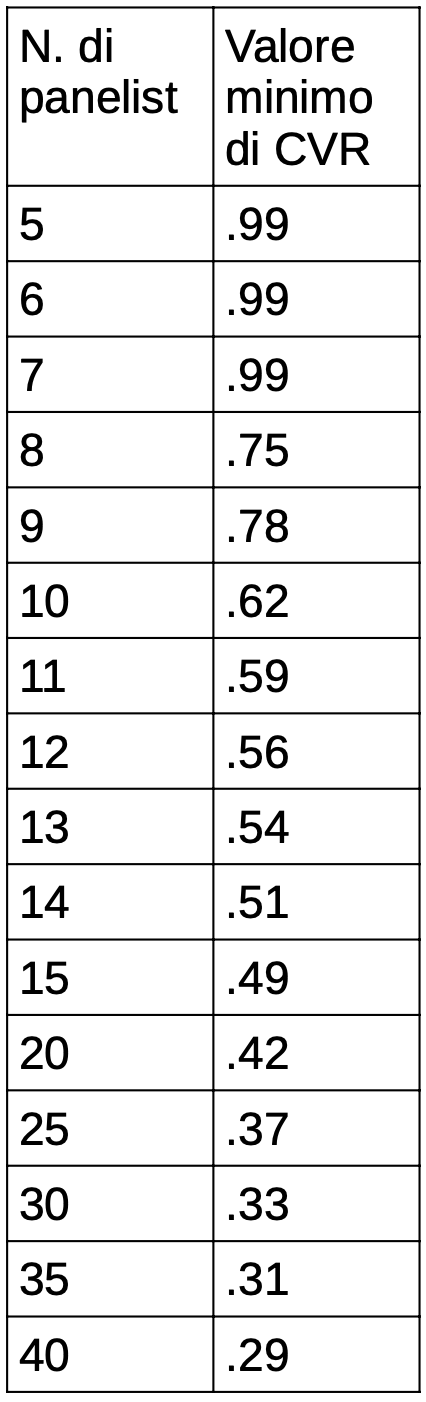
\includegraphics[scale=0.25]{Figures/tab_lawshe.png}
    \end{figure}
\end{columns}

In alternativa si mantengono gli item in cui CVR\textgreater=0.78
(Polit, Becl, Owen, 2007)
\end{frame}

\begin{frame}{Validità di contenuto}
\phantomsection\label{validituxe0-di-contenuto-4}
Metodo di Lawshe (1975)

\textbf{Step 4 (opzionale)}: È possibile calcolare un valore per il test
(\textbf{Content Validity Index}) che non è altro che la
\underline{media} dei CVR di tutti gli items.

\[
CVI = 
\frac{
  \displaystyle
  \sum_{I_1}^{I_k}
  \left(
    \frac{
      n_e - \frac{N}{2}
    }{
      \frac{N}{2}
    }
  \right)
}{
  k
}
\] \[
\small
\begin{aligned}
n_e & = \text{numero di panelist (i.e. esperti) che dicono che quell’item è essenziale} \\
N & = \text{numero totale di panelist} \\
k & = \text{numero degli item} \\
I & = \text{gli item che compongono il test} \\
\end{aligned}
\]
\end{frame}

\begin{frame}{Validità di contenuto}
\phantomsection\label{validituxe0-di-contenuto-5}
Note al Metodo di Lawshe (1975)

È interessante notare come il metodo risponde solo in parte alla domanda
di validità di contenuto.

Il metodo di Lawshe mi dice se un dato item è appropriato per il test,
ma non se il test contiene tutti gli item necessari per i suoi scopi
(nell'articolo originale di Lawshe sono discussi alcuni esempi in cui
gli item da cui si parte sono già stati definiti e il problema è
identificare se sono appropriati).

La validità di contenuto, spesso non è considerata né riportata nei test
(non è molto di moda).
\end{frame}

\begin{frame}{Validità di costrutto}
\phantomsection\label{validituxe0-di-costrutto}
\textbf{Validità di costrutto}: esprime quanto il test misura
effettivamente il costrutto che intende misurare, valutando la coerenza
interna degli item oppure la correlazione con altri test.

La validità di costrutto è valutata in due maniere:

\begin{itemize}
\item
  valutando sei gli \textbf{item} misurano in maniera appropriata il
  costrutto.
\item
  valutando se il \textbf{punteggio totale del
  test}\footnote<.->[frame]{nella maggior parte dei casi, il punteggio
    totale si ottiene sommando gli items (in alcuni casi facendo una
    media).} misuri in maniera appropriata il costrutto (rappresenta
  correttamente il costrutto?).
\end{itemize}
\end{frame}

\begin{frame}{Validità di costrutto}
\phantomsection\label{validituxe0-di-costrutto-1}
\begin{center}
  \textbf{Alpha di Cronbach}
\end{center}
\vspace{2em}

Uno dei classici modi per vedere su tutti gli item di un test si
comportano in maniera coerente è tramite l'utilizzo di metriche come
l'alpha di Cronbach.

Questa però è spesso associata più all'affidabilità (vedi quindi slides
su formule affidabilità).
\end{frame}

\begin{frame}{Validità di costrutto}
\phantomsection\label{validituxe0-di-costrutto-2}
\begin{center}
  \textbf{Analisi fattoriale}
\end{center}

\small

L'analisi statistica più comunemente utilizzata per valutare gli item è
l'analisi fattoriale.

L'analisi fattoriale (nel contesto della teoria dei test) indaga se gli
item di un test si comportano in maniera coerente, dimostrando che essi
misurano uno stessa variabile latente (detto fattore).

Operativamente e per questi scopi l'analisi fattoriale viene condotta in
una matrice \(m x n\), dove \(m\) sono gli item (in riga) ed \(n\) sono
i partecipanti (in colonna).

\begin{center}
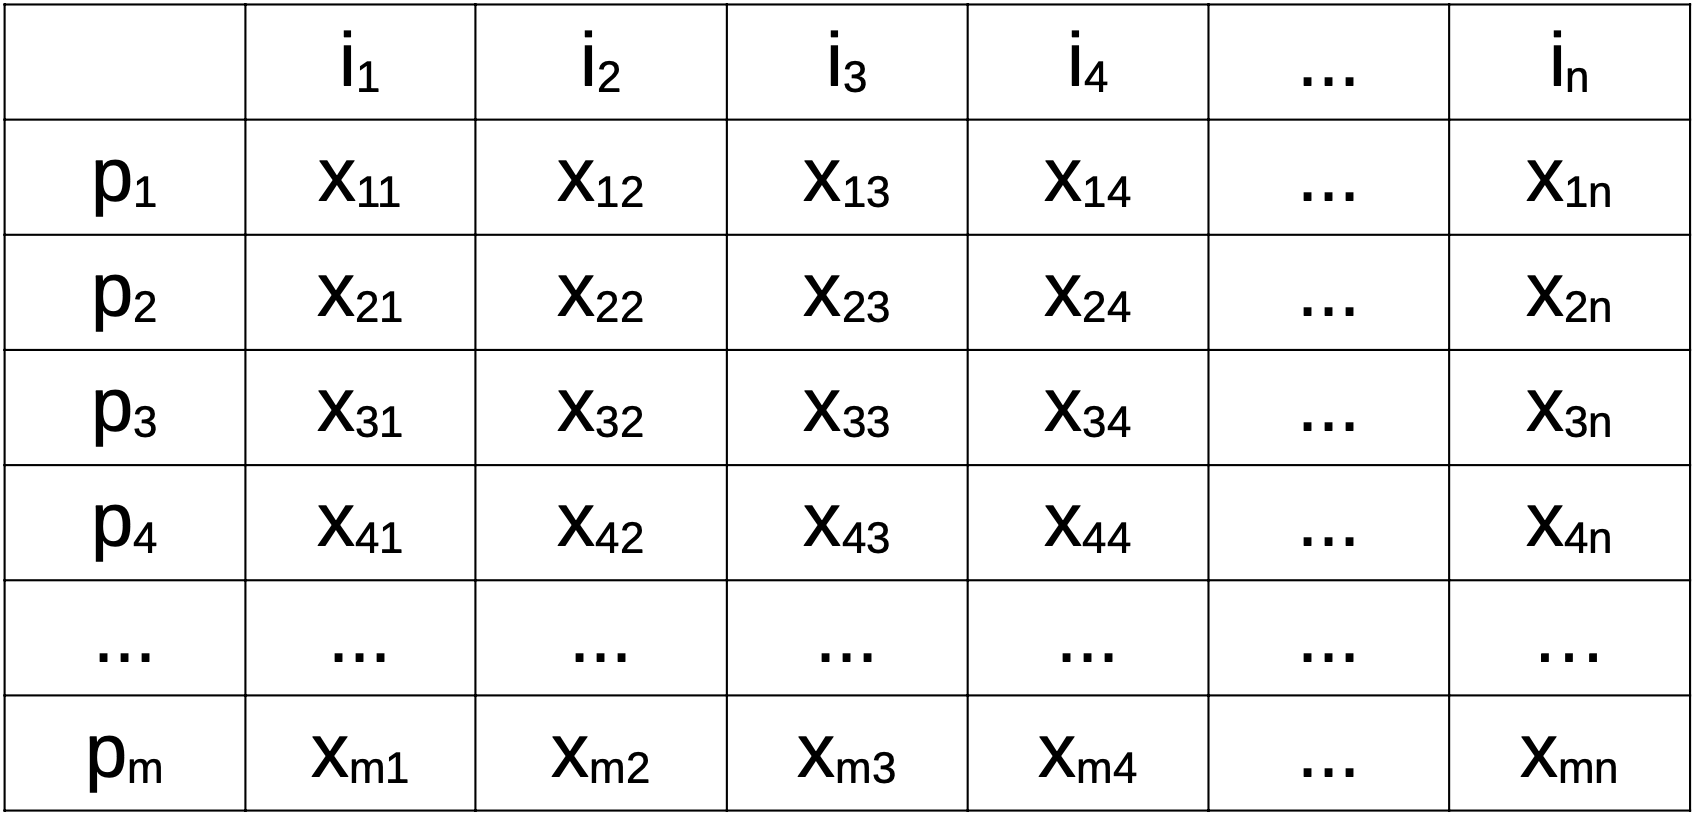
\includegraphics[width=0.5\linewidth,height=\textheight,keepaspectratio]{Figures/fattoriale1.png}
\end{center}
\end{frame}

\begin{frame}{Validità di costrutto}
\phantomsection\label{validituxe0-di-costrutto-3}
\begin{center}
  \textbf{Analisi fattoriale}
\end{center}

Il risultato di un'analisi fattoriale è spesso una matrice di
``loadings'', cioè quanto ciascun item è correlato ad un determinato
fattore. \vspace{1em}

\begin{columns}
  \column{0.5\textwidth}
    \begin{figure}
      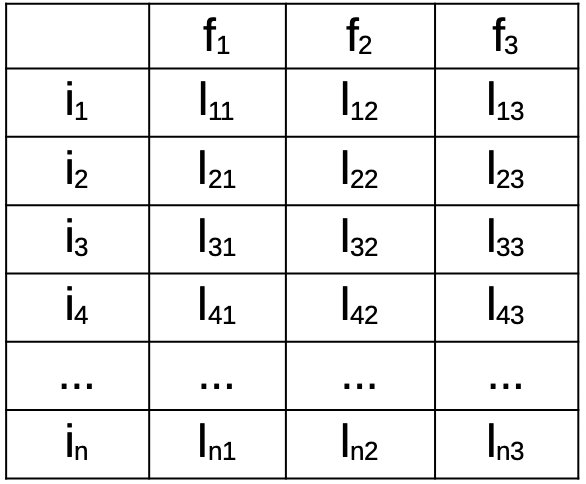
\includegraphics[scale=0.25]{Figures/fattoriale2.png}
    \end{figure}

  \column{0.5\textwidth}
          
      \small
      Esistono delle rule-of-thumb per definire se un loading è significativo (Es. > 0.3 o 0.5 Oppure < -0.3 o -0.5)
      
      i = item
      
      F = fattore
      
      l = loading

\end{columns}
\end{frame}

\begin{frame}{Validità di costrutto}
\phantomsection\label{validituxe0-di-costrutto-4}
\begin{center}
  \textbf{Analisi fattoriale}
\end{center}
\vspace{1em}

In questo esempio gli item caricano su 2 fattori \vspace{1em}

\begin{columns}
  \column{0.3\textwidth}
    \begin{figure}
      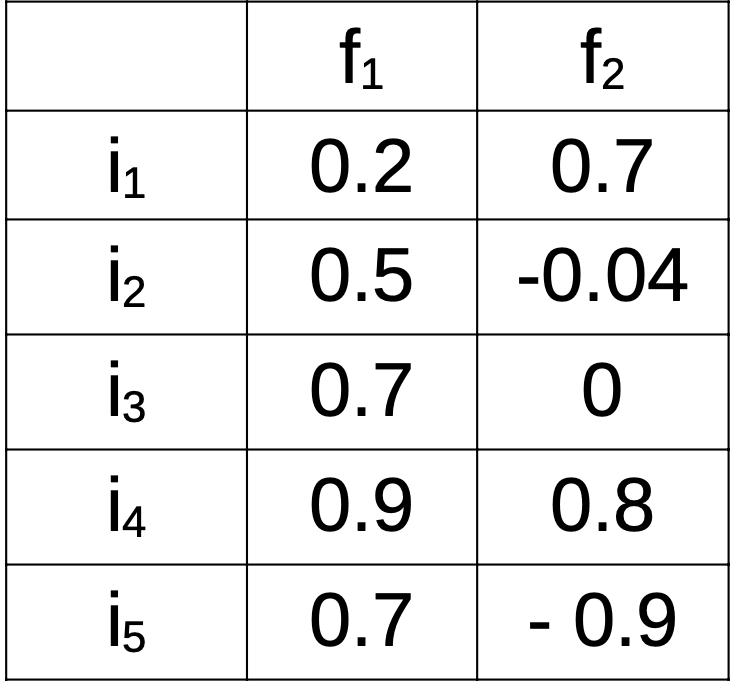
\includegraphics[scale=0.4]{Figures/fattoriale3.png}
    \end{figure}

  \column{0.7\textwidth}
          
      \scriptsize
      Un primo fattore cattura una correlazione positiva tra gli item 1,2,3 che tendono avere punteggi correlati tra loro.\\
\vspace{1em}      
Un secondo fattore cattura una correlazione positiva tra gli item 4,5, che tendono ad avere punteggi correlati tra loro. \\
\vspace{1em}      
Questo è uno scenario ideale, in cui items "caricano" chiaramente in maniera distinta in specifici fattori.


\end{columns}
\end{frame}

\begin{frame}{Validità di costrutto}
\phantomsection\label{validituxe0-di-costrutto-5}
\begin{center}
  \textbf{Analisi fattoriale}
\end{center}
\vspace{1em}

In questo esempio gli item caricano su 2 fattori \vspace{1em}

\begin{columns}
  \column{0.3\textwidth}
    \begin{figure}
      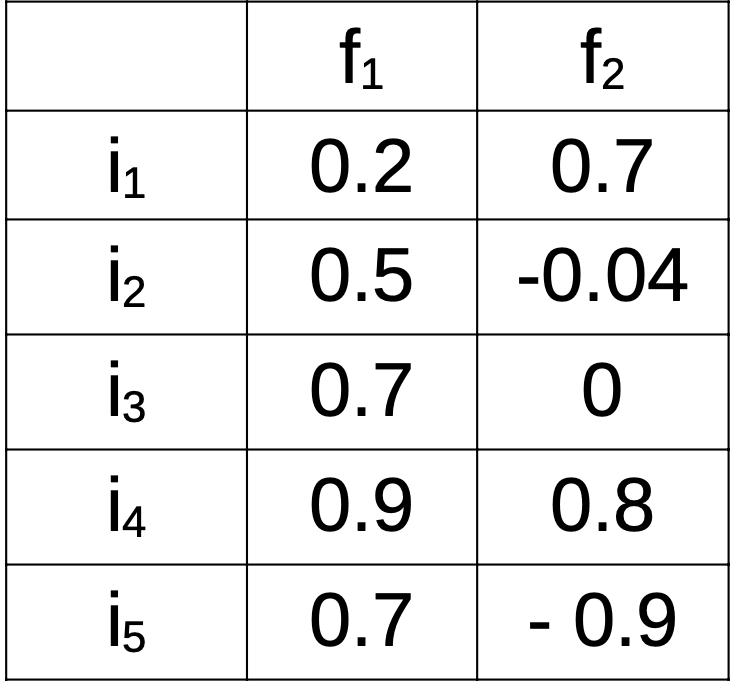
\includegraphics[scale=0.25]{Figures/fattoriale4.png}
    \end{figure}

  \column{0.7\textwidth}
          
      \scriptsize
      Un primo fattore cattura una correlazione positiva tra gli item 2,3,4,5, che tendono avere punteggi tutti correlati tra loro.\\
\vspace{1em}
Un secondo fattore cattura una correlazione negativa di item 1 e 4 rispetto ad item 9. In sostanza quando sono alti i punteggi di 1 e 4 son obassi quelli di 5, e viceversa.\\
\vspace{1em}
Questo è uno scenario più complesso (e comune), il fatto che un item carichi su pià fattori ("cross loadings") può essere indice che l'item non è adeguato o che il modello teorico va rivisto.

\end{columns}
\end{frame}

\begin{frame}{Validità di costrutto}
\phantomsection\label{validituxe0-di-costrutto-6}
\begin{center}
  \textbf{Analisi fattoriale}
\end{center}
\vspace{2em}

Esistono due tipi principali di analisi fattoriale.

L'\textbf{analisi fattoriale esplorativa}, ha come scopo cercare di
definire qual è la struttura fattoriale che meglio descrive (se esiste)
la relazione tra items.

L'\textbf{analisi fattoriale confermativa}, ha come scopo verificare se
gli item si comportano in maniera conforme ad una struttura fattoriale
nota.
\end{frame}

\begin{frame}{Validità di costrutto}
\phantomsection\label{validituxe0-di-costrutto-7}
\begin{center}
  \textbf{Analisi fattoriale}
\end{center}
\vspace{2em}

Nel contesto della validità di costrutto l'analisi fattoriale può essere
una tecnica utilizzata per selezionare gli item che comporranno gli item
del test finale (ad esempio escludendo quelli che non si comportano in
maniera adeguata rispetto al costrutto o ai costrutti che si intendeva
misurare).

Ad esempio, se un test intende misurare un singolo costrutto e tutti gli
item eccetto uno hanno loading alti in un fattore, probabilmente
quell'item andrebbe eliminato dalla versione finale del test.
\end{frame}

\begin{frame}{Validità di costrutto}
\phantomsection\label{validituxe0-di-costrutto-8}
\begin{center}
  \textbf{Analisi fattoriale}
\end{center}
\vspace{2em}

Esistono molte analisi statistiche e metriche per valutare la bontà di
un'analisi fattoriale.

Tra i più comuni si usa il test di Goodness-of-Fit (è un test che
riporta Chi-quadro) che deve essere \textbf{non significativo (p
\textgreater{} 0.05)}. Se significativo vuol dire che la struttura a
fattori proposta non è sufficiente per spiegare la variabilità dei dati.

Altre metriche sono il \textbf{RMSEA} (root Mean squared error of
Approximation) che deve essere il più basso possibile (di solito
\textless0.06 è considerata una soglia minima).
\end{frame}

\begin{frame}{Validità di costrutto}
\phantomsection\label{validituxe0-di-costrutto-9}
\begin{center}
  \textbf{Analisi fattoriale}
\end{center}
\vspace{1em}

\begin{columns}
  \column{0.4\textwidth}
  
    L’analisi fattoriale è spesso rappresentata in maniera grafica distinguendo i fattori latenti (in questo caso cerchi) dalle variabili osservate (in questo caso quadrati).

  \column{0.6\textwidth}
    \begin{figure}
      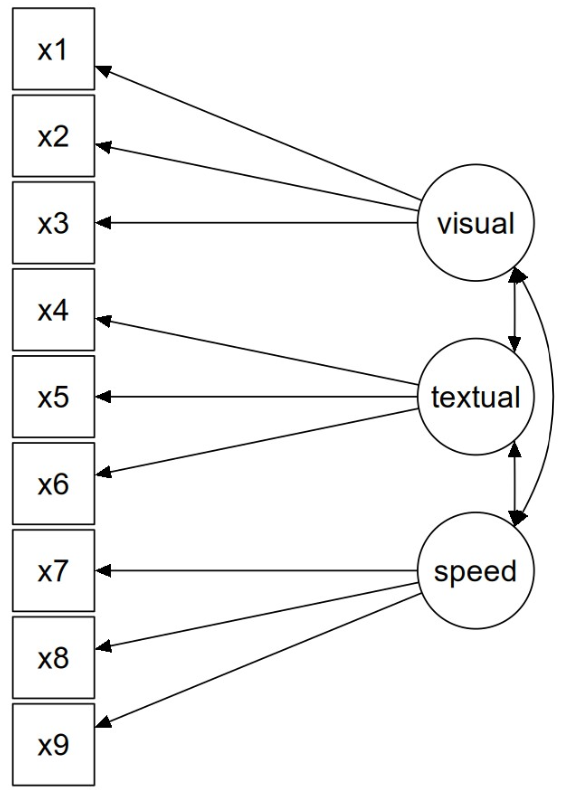
\includegraphics[scale=0.4]{Figures/fattoriale5.png}
    \end{figure}
    
    \small
      \href{https://lavaan.ugent.be/tutorial/cfa.html}{\underline{https://lavaan.ugent.be/tutorial/cfa.html}}

\end{columns}
\end{frame}

\begin{frame}{Validità di costrutto}
\phantomsection\label{validituxe0-di-costrutto-10}
\begin{center}
  \textbf{Analisi fattoriale}
\end{center}
\vspace{1em}

Per interpretare se un'analisi fattoriale supporta effettivamente la
validità di costrutto, andrebbe visto se gli item si comportano
effettivamente come il test assume si dovrebbero comportare.

Es. se un test sostiene di misurare un costrutto specifico (es.
Attenzione visuospaziale) tutti gli item dovrebbero caricare su un solo
fattore (almeno principalmente).

È innanzitutto utile vedere se gli autori di un test hanno effettuato
analisi fattoriale per indagare la relazione tra gli item e li hanno
selezionati (escludendone alcuni) o in generale se c'è stata una qualche
fase di selezione degli items (es. item selection tramite correlazione).
\end{frame}

\begin{frame}{Validità di costrutto}
\phantomsection\label{validituxe0-di-costrutto-11}
\begin{center}
  \textbf{Analisi fattoriale}
\end{center}
\vspace{1em}

Stabilire l'adeguatezza di un'analisi fattoriale non è comunque semplice
perché spesso è possibile fare giustificazioni solo a posteriori dei
risultati finali, senza che i risultati abbiano influenzato la scelta se
tenere o meno degli items.

Ad esempio, potrei avere un test che assume di misurare uno specifico
costrutto, trovare con un'analisi fattoriale esplorativa che in realtà
la variabilità degli item è spiegata da \emph{due} fattori e mantenere
comunque tutti gli item dicendo che probabilmente sono influenzati da
due fattori separati, coerenti con aspettative da teoria (Es. Attenzione
visuospaziale e funzioni esecutive).
\end{frame}

\begin{frame}{Validità di costrutto}
\phantomsection\label{validituxe0-di-costrutto-12}
\begin{center}
  \textbf{Analisi fattoriale}
\end{center}
\vspace{2em}

Nota che a volte l'analisi fattoriale è usata anche per i punteggi di
sottoscale che compongono una batteria (es. Per APACS, Arcara \& Bambini
2016).

I principi sono gli stessi, ma in questo caso non si tratta di items, ma
di gruppi di items che compongono sottoscale (in questo caso es. il task
di Linguaggio Figurato 1, il task di Linguaggio Figurato 2 etc.).
\end{frame}

\begin{frame}{Validità di costrutto}
\phantomsection\label{validituxe0-di-costrutto-13}
\begin{center}
  \textbf{Principal Component Analysis (PCA)}
\end{center}

\small

PCA e analisi fattoriale sono concettualmente simili e i risultati (una
matrice di loadings) sono anch'essi simili. La differenza è che nella
PCA non c'è stima di ``variabili latenti'', ma lo scopo è \emph{ottenere
nuove variabili che catturano porzioni di varianza comune tra più
punteggi} (es. items, o punteggi totali di test). Tali variabili sono
dette \textbf{componenti principali} (da cui il nome dell'analisi).
Questa differenza si riflette in una diversità a livello della formula e
nei risultati che si otterranno.

Quindi potreste trovare in un test una PCA invece di un'analisi
fattoriale. Potete interpretarle in maniera analoga, anche se sarebbe
più corretto utilizzare l'analisi fattoriale perchè assume l'esistenza
di variabili latenti, cosa che è spesso implicita quando si tratta di
item o punteggi totali di test psicologici.
\end{frame}

\begin{frame}{Validità di costrutto}
\phantomsection\label{validituxe0-di-costrutto-14}
\begin{center}
  \textbf{Nota Analisi Fattoriale e PCA}
\end{center}

\small

Analisi fattoriale e PCA ci aiutano a capire come si raggruppano gli
items e se lo fanno in maniera coerente con il costrutto (o i costrutti)
che dovrebbero misurare.

Non ci garantiscono però che il costrutto sia quello giusto e pertanto
sono solo un'informazione parziale sulla validità.

Ad esempio, immaginiamo che voglia valutare validità di costrutto di un
test di memoria. Gli autori potrebbero riportare un'analisi fattoriale
che mostra che gli item correlano bene fra di loro e sono riconducibili
a un'unica variabile latente. Questo è ottimo ma \emph{non mi garantisce
che questa variabile latente sia effettivamente la memoria}. Il test
potrebbe essere stato costruito in maniera sbagliata e gli item essere
consistenti per un altro motivo (es. magari il test cattura perlopiù
velocità psicomotoria).
\end{frame}

\begin{frame}{Validità di costrutto}
\phantomsection\label{validituxe0-di-costrutto-15}
\begin{center}
  \textbf{Correlazione}
\end{center}

Lo strumento più comune per verificare la validità di costrutto di un
test è indagare la correlazione del punteggio totale al test con
correlazione dei punteggi ad altri test.

Non esiste una regola di quanto dovrebbe essere almeno questa
correlazione, ma è ragionevole pensare che debba essere almeno moderata
(\textgreater{} 0.3), ma verosimilmente anche di più.

I test neuropsicologici (specie nei sani) tendono sempre ad essere
\textbf{molto correlati fra di loro} e correlazioni più alte sono attese
(di fatto queste correlazioni hanno portato ad ipotizzare al cosiddetto
fattore g dell'intelligenza)

\href{https://en.wikipedia.org/wiki/G_factor_(psychometrics)}{\ul{https://en.wikipedia.org/wiki/G\_factor\_(psychometrics)}}
\end{frame}

\begin{frame}{Validità di costrutto}
\phantomsection\label{validituxe0-di-costrutto-16}
\begin{center}
  \textbf{Correlazione}
\end{center}
\vspace{1em}

\begin{columns}
  \column{0.5\textwidth}
    \begin{figure}
      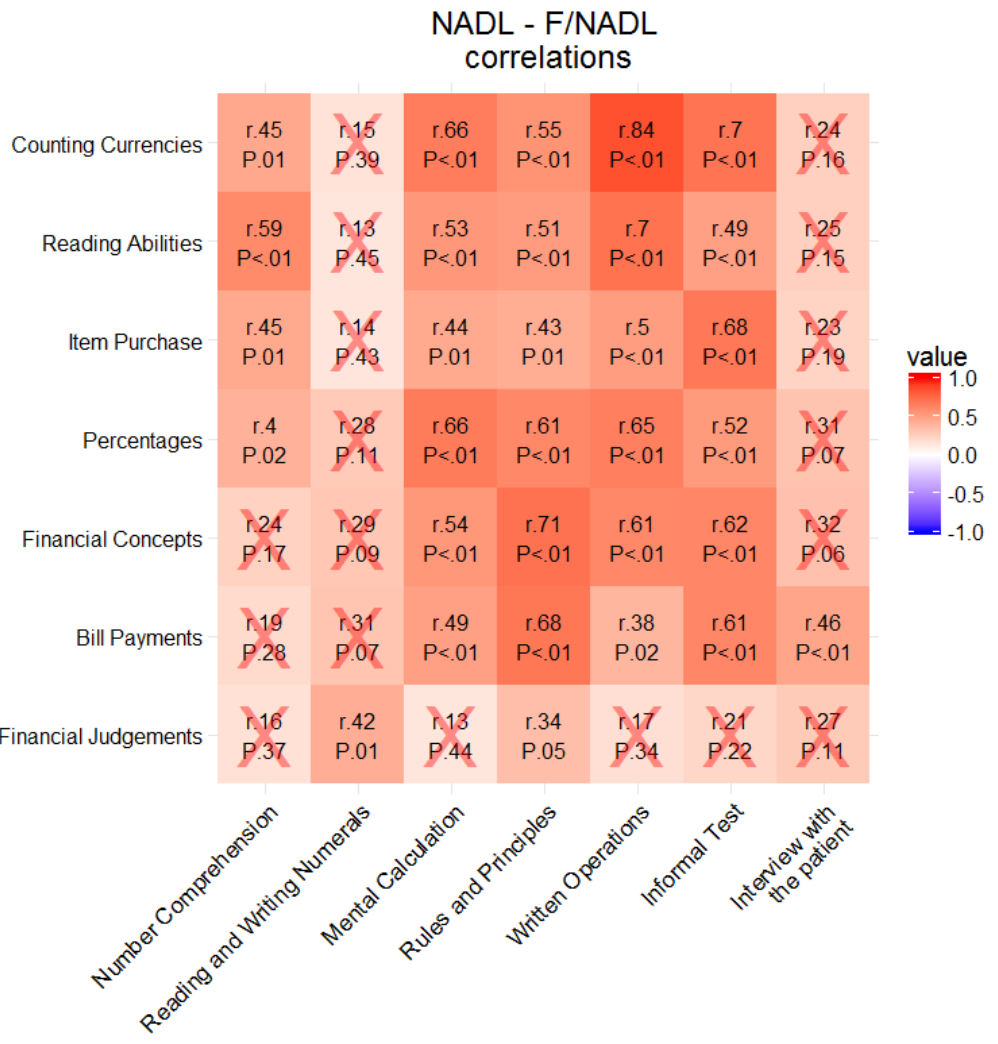
\includegraphics[scale=0.3]{Figures/correlazione.png}
    \end{figure}

  \column{0.5\textwidth}
    Questa figura riporta le correlazioni tra alcuni test del NADL (Semenza et al., 2014) e il NADL-F (Arcara et al., 2019).

\end{columns}
\end{frame}

\begin{frame}{Validità di costrutto}
\phantomsection\label{validituxe0-di-costrutto-17}
\begin{center}
  \textbf{Correlazione}
\end{center}
\vspace{2em}

L'aspetto critico dell'interpretare valori ``soglia'' di correlazioni
tra due diversi test è che i valori sono anche legati ai rispettivi
errori dei test (quindi ad aspetti legati a numerosità campionarie e
affidabilità, vedi future slides).

Inoltre è sempre possibile ``giustificare'' a posteriori un'eventuale
differenza o valore basso (es. La correlazione è bassa presumibilmente
perchè questo test implica di più le funzioni esecutive rispetto
all'altro).
\end{frame}

\begin{frame}{Validità di costrutto}
\phantomsection\label{validituxe0-di-costrutto-18}
\begin{center}
  \textbf{Correlazione}
\end{center}
\vspace{2em}

Anche l'assenza di correlazione o correllazione molto bassa può essere
usata a sostegno di una buona validità di costrutto.

In generale la validità di costrutto indica quanto bene stiamo misurando
lo specifico costrutto.

Dimostrare che stiamo isolando bene la specifica funzione cognitiva è a
sostegno della validità di costrutto.
\end{frame}

\begin{frame}{Validità di costrutto}
\phantomsection\label{validituxe0-di-costrutto-19}
\begin{center}
  \textbf{Correlazione}
\end{center}
\vspace{1em}

\begin{columns}
  \column{0.5\textwidth}
    \begin{figure}
      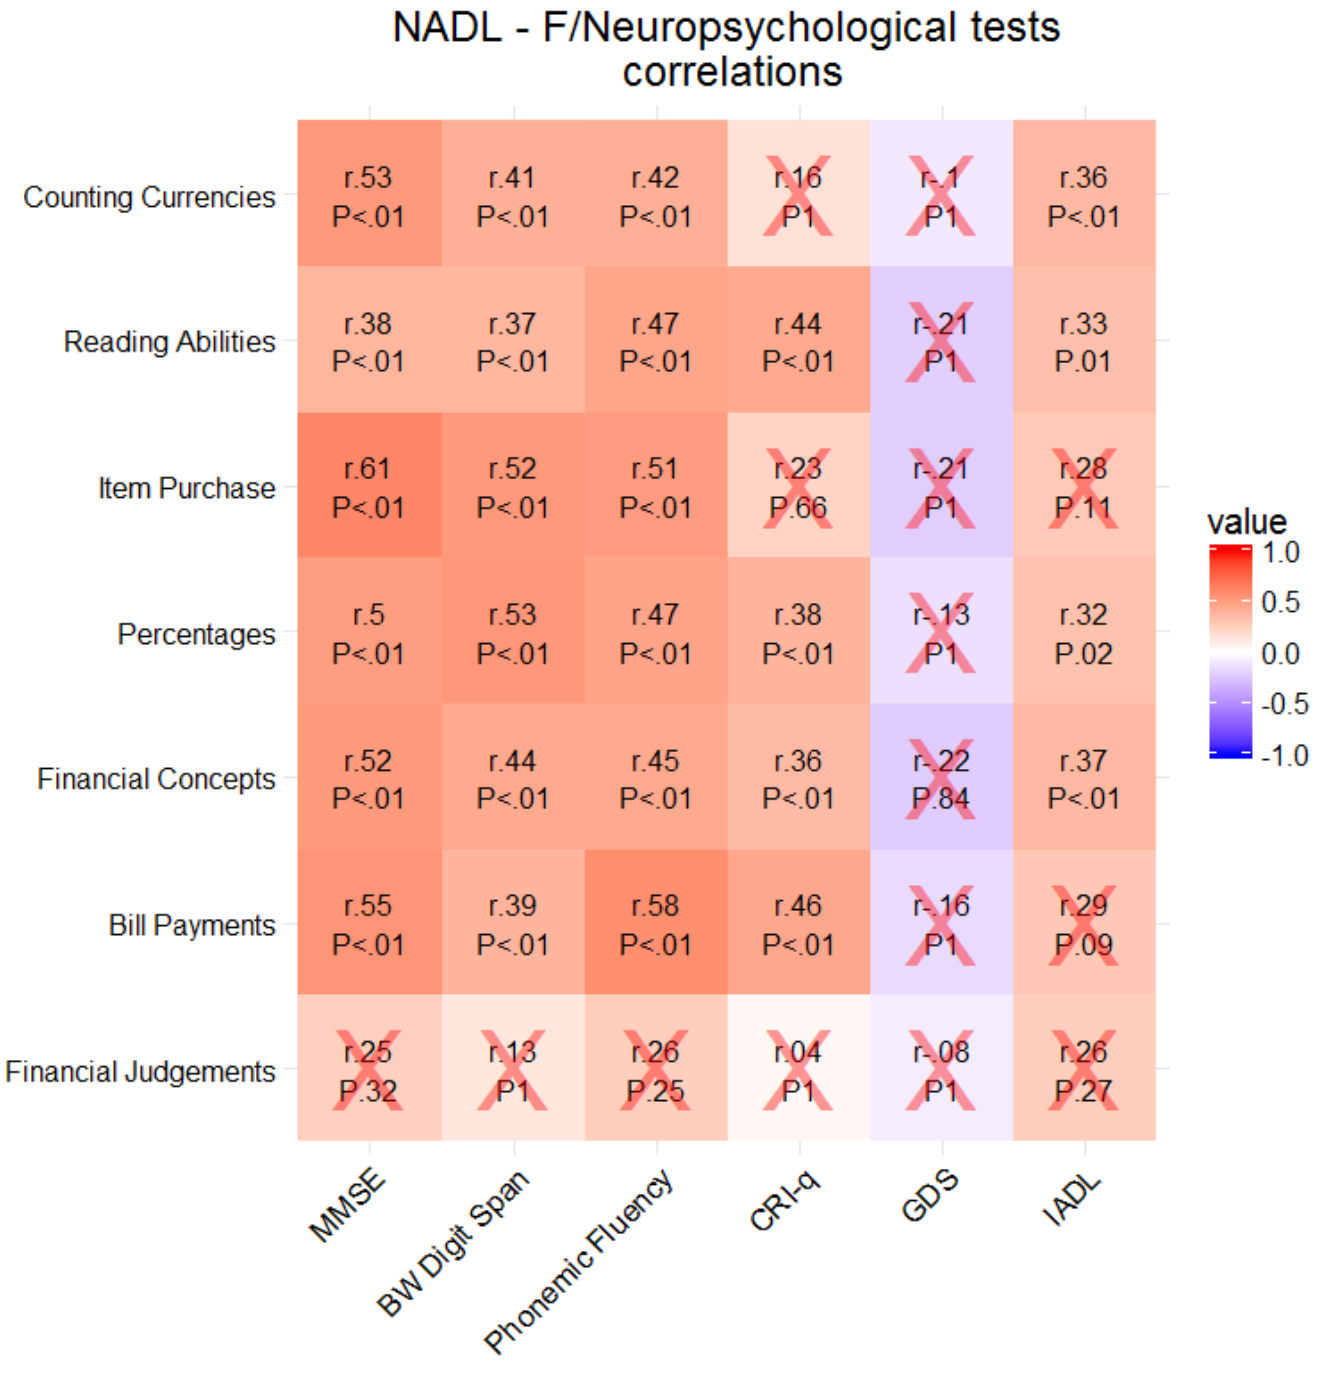
\includegraphics[scale=0.25]{Figures/correlazione2.png}
    \end{figure}

  \column{0.5\textwidth}
  \small
   Questa figura riporta le correlazioni tra alcuni test di vario tipo e il NADL-F (Arcara et al., 2019).
   
   Notate che non correla con GDS (geriatric Depression Scales), a sostegno della sua validità di costrutto.

\end{columns}
\end{frame}

\begin{frame}{Validità di costrutto}
\phantomsection\label{validituxe0-di-costrutto-20}
\begin{center}
  \textbf{Altre analisi}
\end{center}

\small

In generale la validità di costrutto non è vincolata a specifiche
analisi statistiche e andrebbe valutata rispetto alla specifica domanda
a cui cerca di rispondere. In altre parole, piuttosto che cercare nei
manuali / articoli specifiche analisi (es. È stata fatta analisi
fattoriale? Ci sono correlazioni?), dovreste cercare di rispondere a
questa domanda:

\emph{Esistono evidenze sperimentali che suggeriscono che il test stia
misurando quello che intende misurare?}

Ad esempio un test che ha come obiettivo valutare la capacità di
lavorare potrebbe non avere nessuna correlazione con altri test, ma
essere buono nel discriminare persone che sono state licenziate, da
quelle che hanno mantenuto il lavoro (in questo caso una regressione
logistica o altre analisi più legate alla discriminazione).
\end{frame}

\begin{frame}{Validità di costrutto}
\phantomsection\label{validituxe0-di-costrutto-21}
\begin{center}
  \textbf{Altre analisi}
\end{center}
\vspace{1em}

Esempio da Kershaw \& Webber, 2008 \vspace{1em}

\begin{columns}
  \column{0.5\textwidth}
    \begin{figure}
      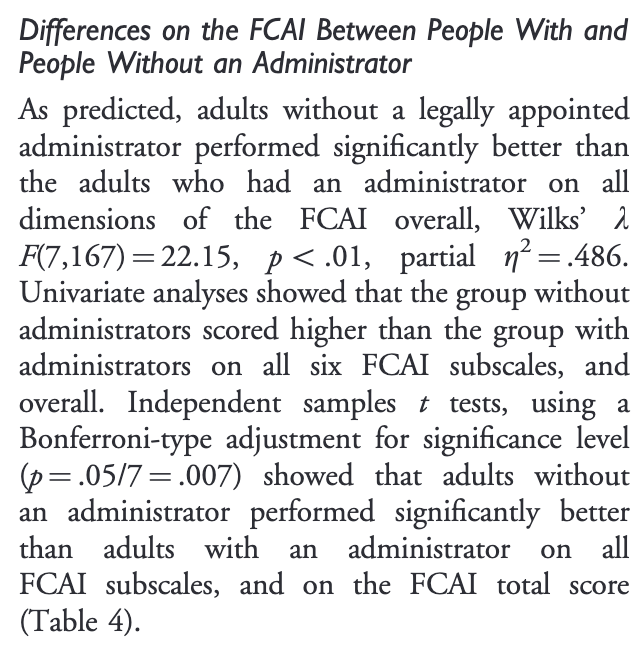
\includegraphics[scale=0.4]{Figures/FCAI.png}
    \end{figure}

  \column{0.5\textwidth}
   Il FCAI è un test per valutazione competenze finanziarie. Per dimostrare validità di costrutto sono stati confrontati partecipanti con e senza tutore legale (tramite MANOVA).

\end{columns}
\end{frame}

\begin{frame}{Validità di costrutto}
\phantomsection\label{validituxe0-di-costrutto-22}
\begin{center}
  \textbf{Altre analisi}
\end{center}

\small

È possibile anche combinare analisi precedentemente citate per
supportare validità di costrutto.

Ad esempio Montemurro et al.~(2023) per dimostrare che il test Tele-GEMS
era utile per valutare cognizione generale hanno usato il seguente
approccio:

\begin{enumerate}
[1)]
\item
  raccolto dati su pazienti (Sclerosi Multipla in quel caso), su vari
  test.
\item
  fatto PCA su questi test e ottenuto un punteggio globale (prima
  componente) che catturava il 60\% della varianza.
\item
  visto se punteggio Tele-GEMS correlava con questo punteggio. La
  correlazione era 0.50 (moderata/alta) e interepretata a supporto di
  una buona validità di costrutto del test.
\end{enumerate}
\end{frame}

\begin{frame}{Validità di costrutto}
\phantomsection\label{validituxe0-di-costrutto-23}
\begin{center}
  \textbf{Altre analisi}
\end{center}
\vspace{2em}

Un altro ipotetico esempio su come combinare analisi per validità di
costrutto:

Se l'analisi fattoriale mostra che gli item si comportano come se
catturassero due variabili latenti, una associata ad attenzione ed una a
memoria, sarebbe utile e a supporto di validità di costrutto se i
punteggi ottenuti sommando queste due parti correlassero rispettivamente
con un altro test di attenzione ed un altro test di memoria.
\end{frame}

\section{Validità di criterio}\label{validituxe0-di-criterio}

\begin{frame}{Validità di criterio}
\phantomsection\label{validituxe0-di-criterio-1}
La \textbf{validità di criterio} valuta quanto un test è associato o
predice un altra variabile di outcome (osservabile), detta
gold-standard.

Le analisi che si possono utilizzare e come valutare i risultati
cambiano a seconda che il criterio sia una variabile continua (es. Il
punteggio ad un altro test) oppure una variabile categoriale (es.
l'appartenza ad un gruppo, es MCI vs Controlli).
\end{frame}

\begin{frame}{Validità di criterio}
\phantomsection\label{validituxe0-di-criterio-2}
\begin{center}
  \textbf{Variabile continua}
\end{center}

Se il gold standard è una variabile continua, allora si può vedere
tramite una correlazione. In tal caso la correlazione dovrebbe essere
molto alta (\textgreater{} 0.9).

A partire dalla correlazione possiamo calcolare la varianza spiegata
(nota anche come \(r^2\)) che non è altro che il coefficiente di
correlazione al quadrato.

A volte per calcolare la validità di criterio si usa la regressione
lineare. Nel caso di due variabili la regressione lineare è strettamente
imparentata con il coefficiente di correlazione (e infatti i risultati
di alcuni aspetti sono matematicamente identici).
\end{frame}

\begin{frame}{Validità di criterio}
\phantomsection\label{validituxe0-di-criterio-3}
\begin{center}
  \textbf{Variabile categoriale}
\end{center}

\small

Nel caso di variabili categoriali (Es. sopra/sotto cut-off, oppure MCI
vs Controlli), esistono famiglie di analisi diverse che vengono
utilizzate. La categoria più rilevante (spesso patologica) è detta anche
condizione di interesse.

In questa fase diciamo solo che esistono 4 tipi di possibili risultati
quando si confronta un test con il suo criterio (categoriale)

\begin{center}
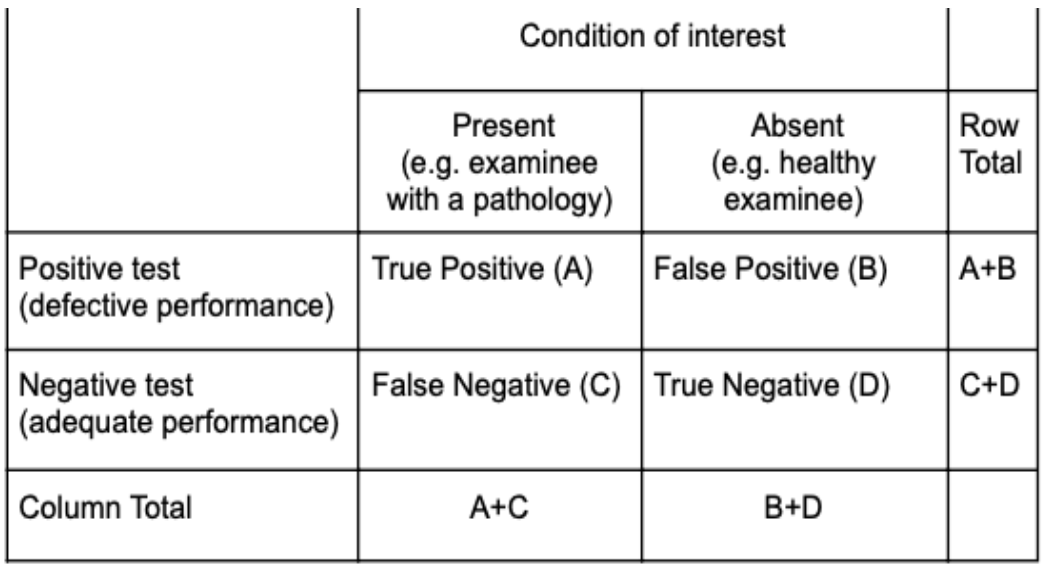
\includegraphics[width=0.5\linewidth,height=\textheight,keepaspectratio]{Figures/variabile_categoriale_costrutto.png}
\end{center}
\end{frame}

\begin{frame}{Validità di criterio}
\phantomsection\label{validituxe0-di-criterio-4}
\begin{center}
  \textbf{Variabile categoriale}
\end{center}
\vspace{2em}

\begin{center}
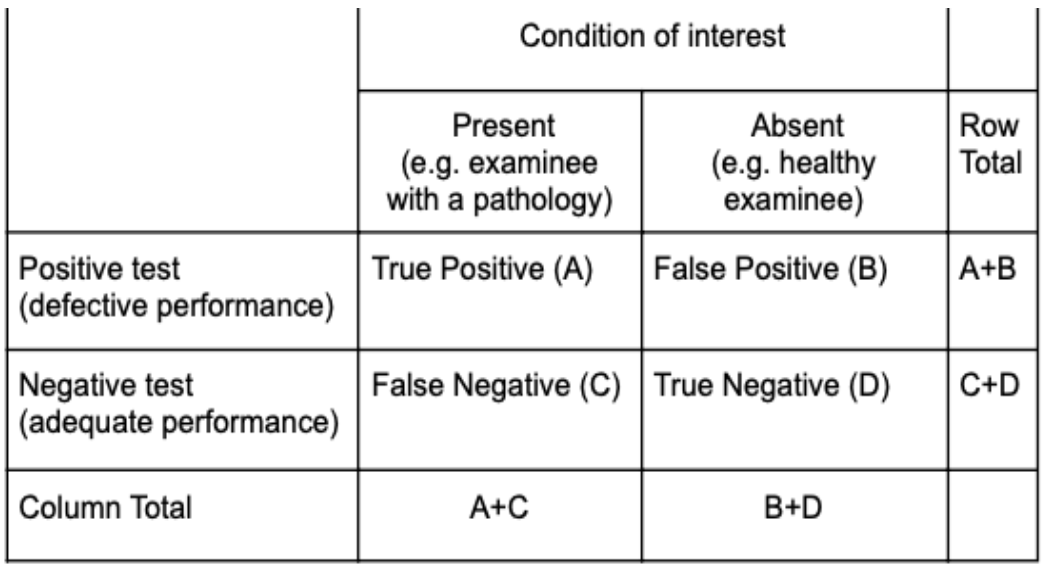
\includegraphics[width=0.5\linewidth,height=\textheight,keepaspectratio]{Figures/variabile_categoriale_costrutto.png}
\end{center}

Tutte le metriche legate a questo fanno parte dei concetti di
Sensibilità/Specificità che saranno trattate in apposite lezioni (dopo i
cut-off)
\end{frame}

\section{Validità di facciata}\label{validituxe0-di-facciata}

\begin{frame}{Validità di facciata}
\phantomsection\label{validituxe0-di-facciata-1}
La \textbf{validità di facciata} valuta quanto un test \emph{sembra}
misurare ciò che intende misurare. \vspace{2em}

\begin{columns}
\column{0.8\textwidth}
\small
Spesso è valutata tramite domande ad hoc ad esperti o tramite confronto con test gold standard esistenti, ma solo tramite confronto qualitativo.

Talvolta la sola informazione che si ha a disposizione di un test è proprio la validità di facciata. Non ci sono altre prove che il test misuri ciò che vuole misurare se non il fatto che sia costruito da item che plausibilimente misurano proprio quel costrutto. 

\column{0.2\textwidth}
\begin{figure}

\includegraphics[scale=0.05]{Figures/triangle.png}
\end{figure}
\end{columns}
\end{frame}

\section{Validità ecologica}\label{validituxe0-ecologica}

\begin{frame}{Validità ecologica}
\phantomsection\label{validituxe0-ecologica-1}
La \textbf{validità ecologica} valuta quanto un test è in grado di
prevedere comportamenti al di fuori del setting di valutazione (quindi
nella vita quotidiana).

Spesso è studiata tramite correlazioni con altre scale riferite a
comportamenti della vita quotidiana (diversamente da molti test
l'interesse non è in costrutti ma in \emph{altri comportamenti}).

Può essere anche essere valutata tramite altre analisi, purché mostrino
che i punteggi al test siano associati al fenomeno di vita quotidiana di
interesse.
\end{frame}




\end{document}
